\begin{frame}
    \begin{center}
        \vspace{3.0cm}
        \normalsize
        \textbf{Игровые программы. Основы проектирования.} \\
        \vspace{1.5cm}
        \raggedleft\small\textbf{Выполнил:}\\Голубев~А.~В.\\САПР-1.1п\\
        \vspace{1.8cm}
        \vspace{\fill}
        \centeringВолгоград \the\year
    \end{center}
\end{frame}

\begin{frame}
    Оглавление:
    \tableofcontents
\end{frame}

\section{Введение}
\begin{frame}
    \frametitle{Введение}
    \raggedleftКомпьютерные игры -- это искусство.
    \begin{figure}
        \begin{minipage}{0.47\textwidth}
            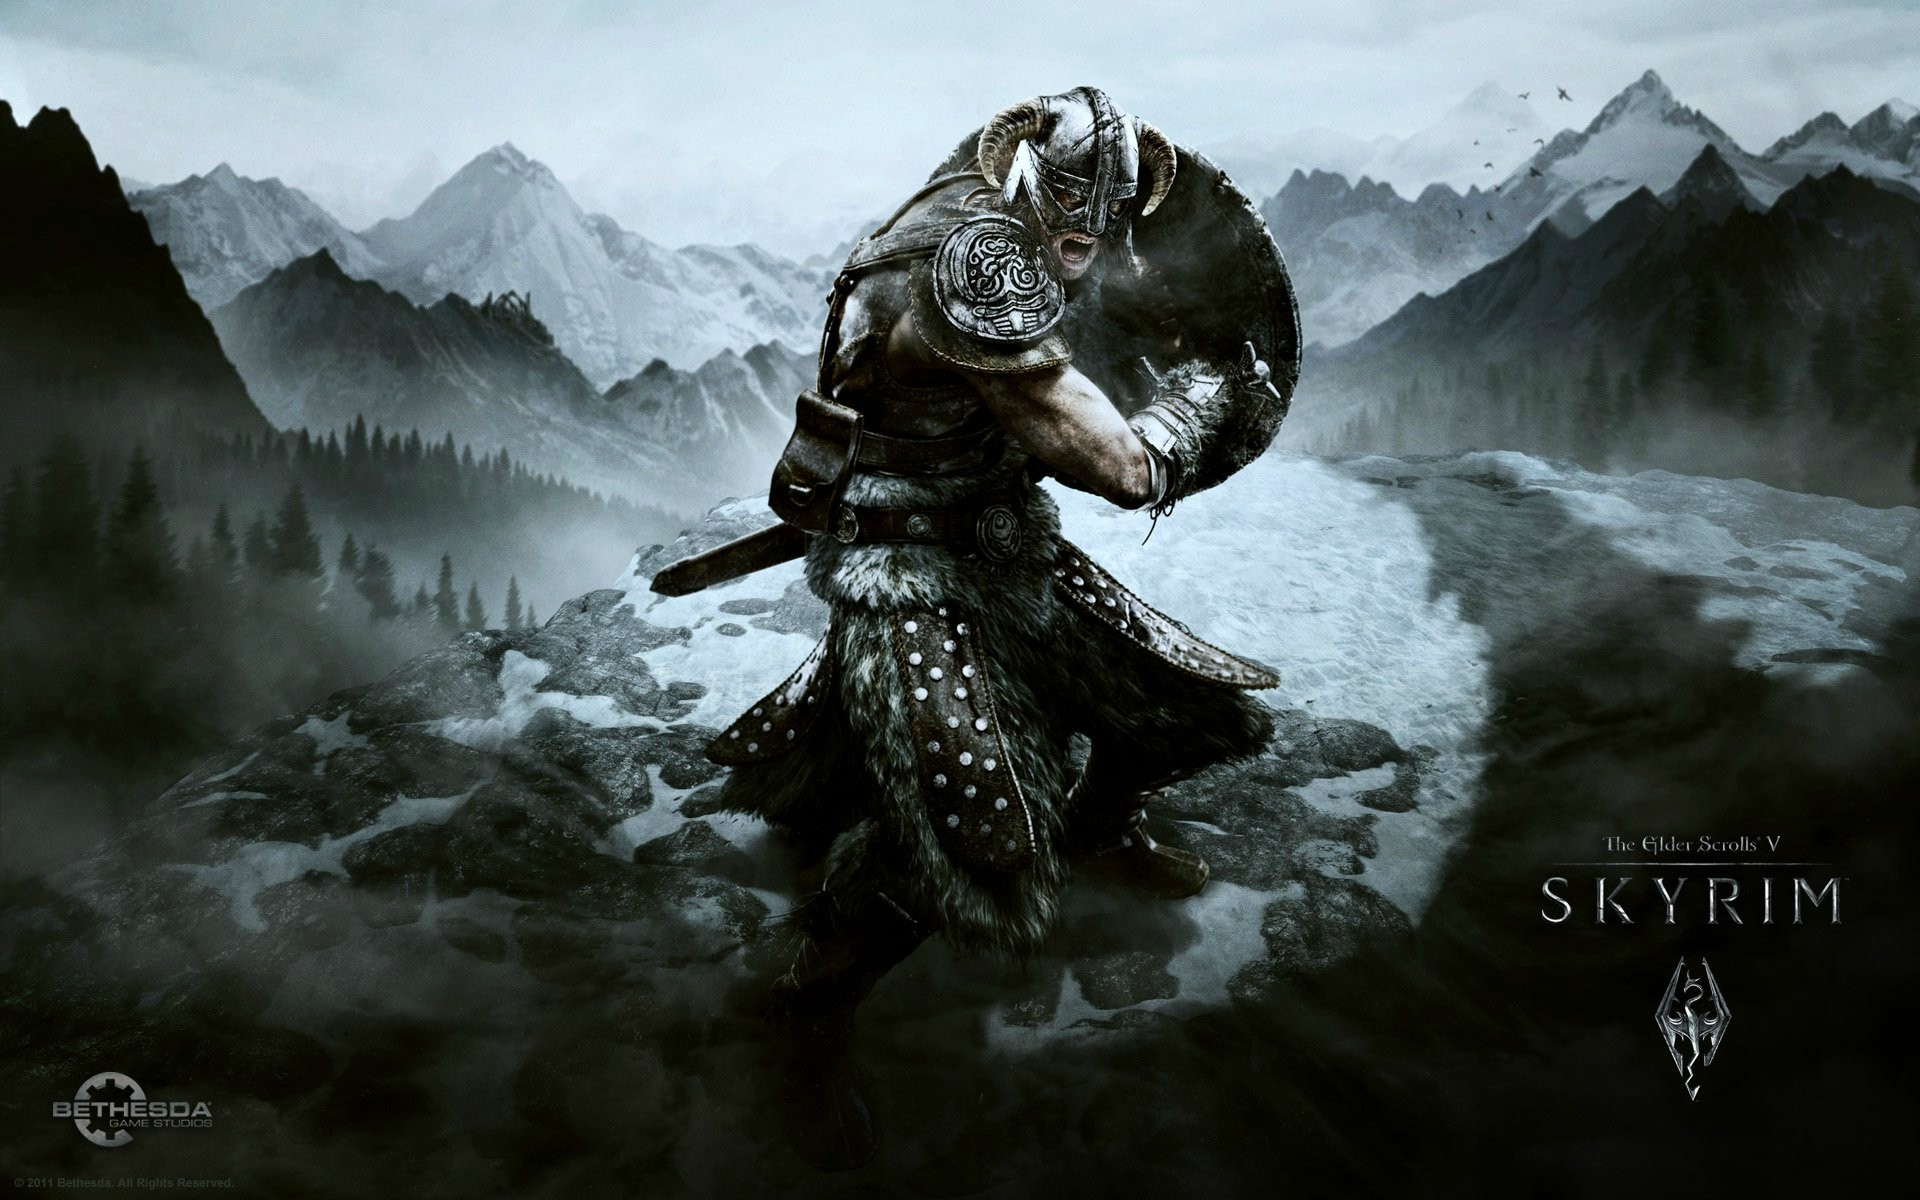
\includegraphics[width=1.0\textwidth]{skyrim}
        \end{minipage}
        \begin{minipage}{0.51\textwidth}
            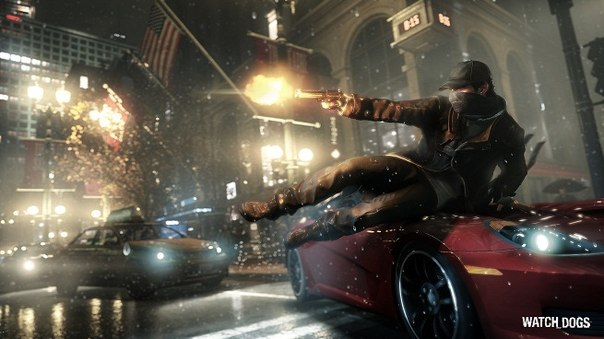
\includegraphics[width=1.0\textwidth]{watch_dogs}
        \end{minipage}
        \begin{minipage}{0.47\textwidth}
            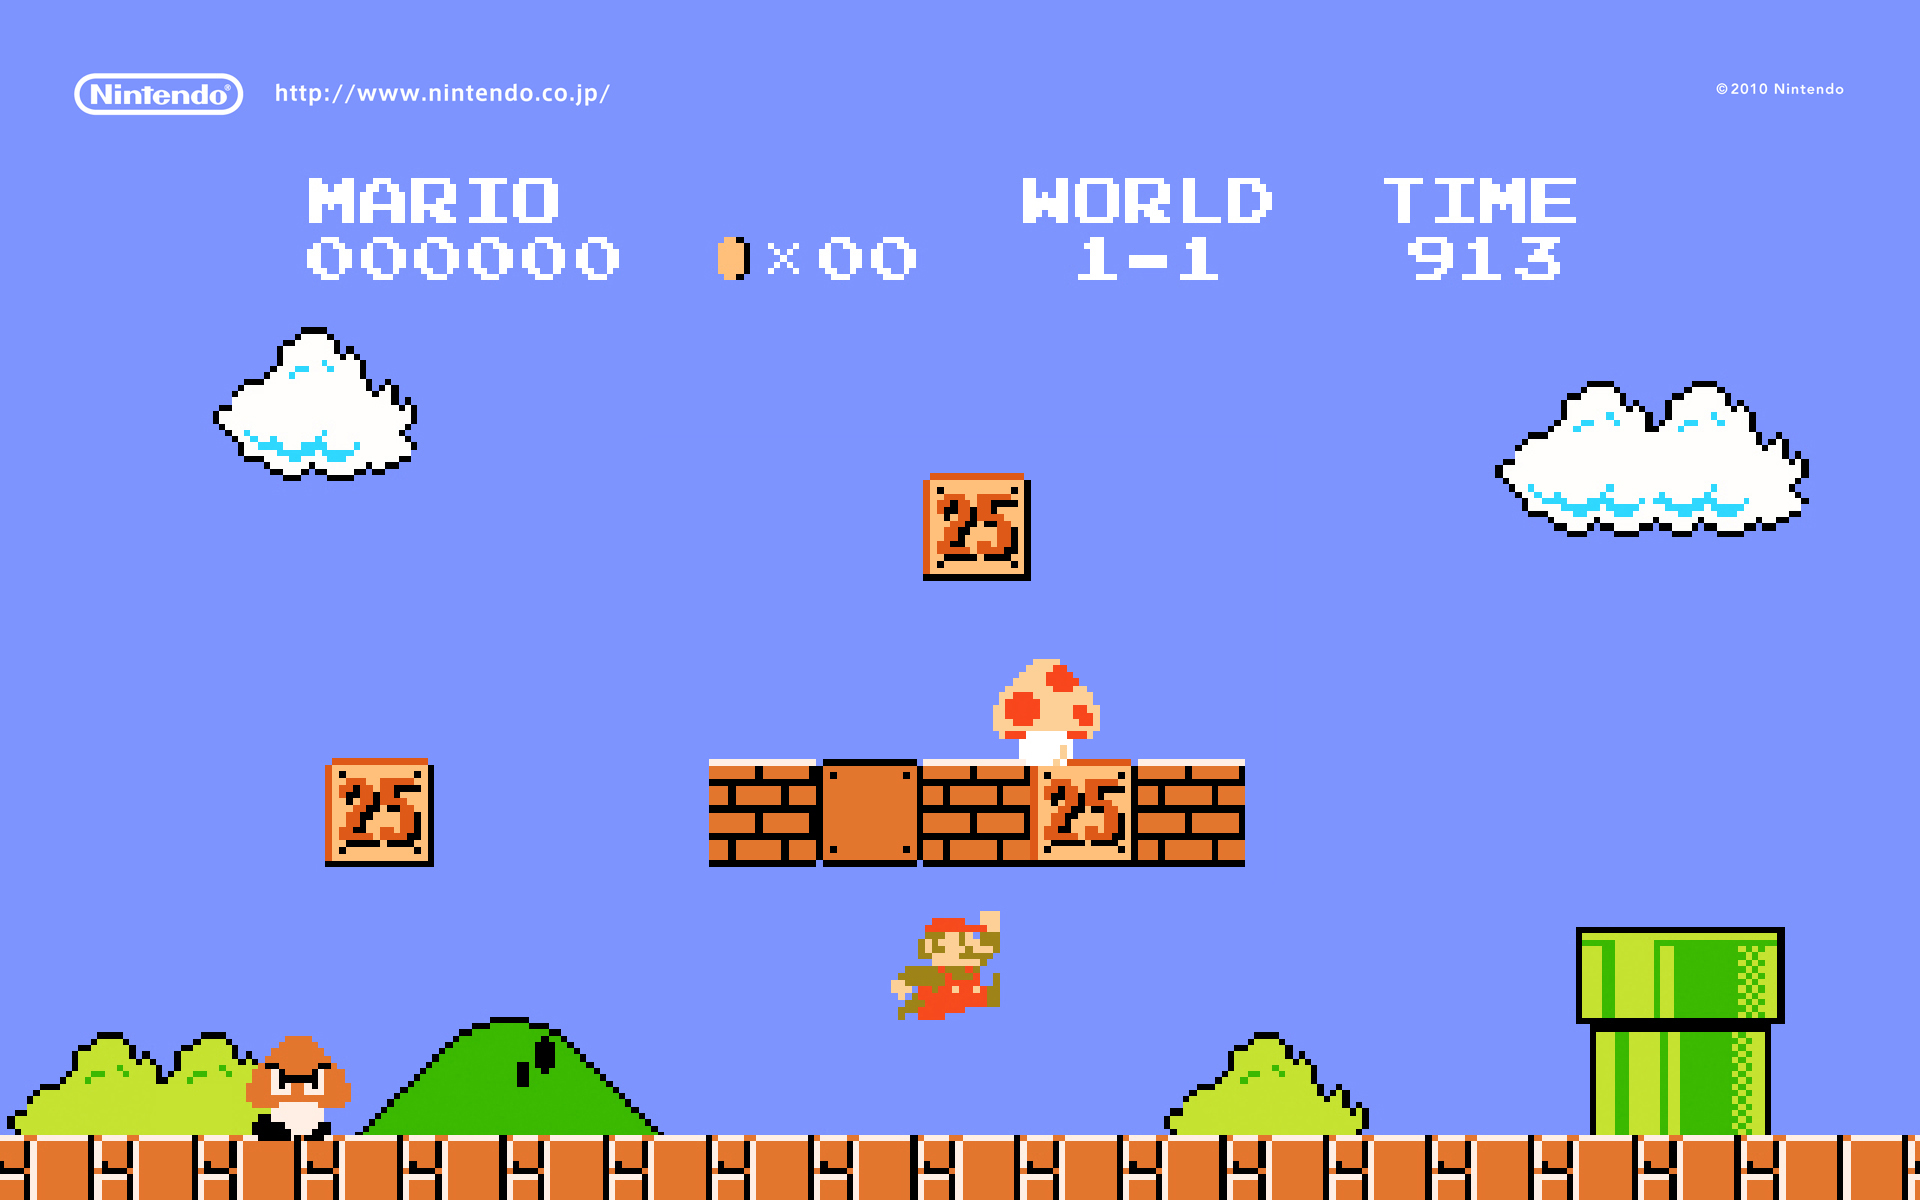
\includegraphics[width=1.0\textwidth]{mario}
        \end{minipage}
        \begin{minipage}{0.51\textwidth}
            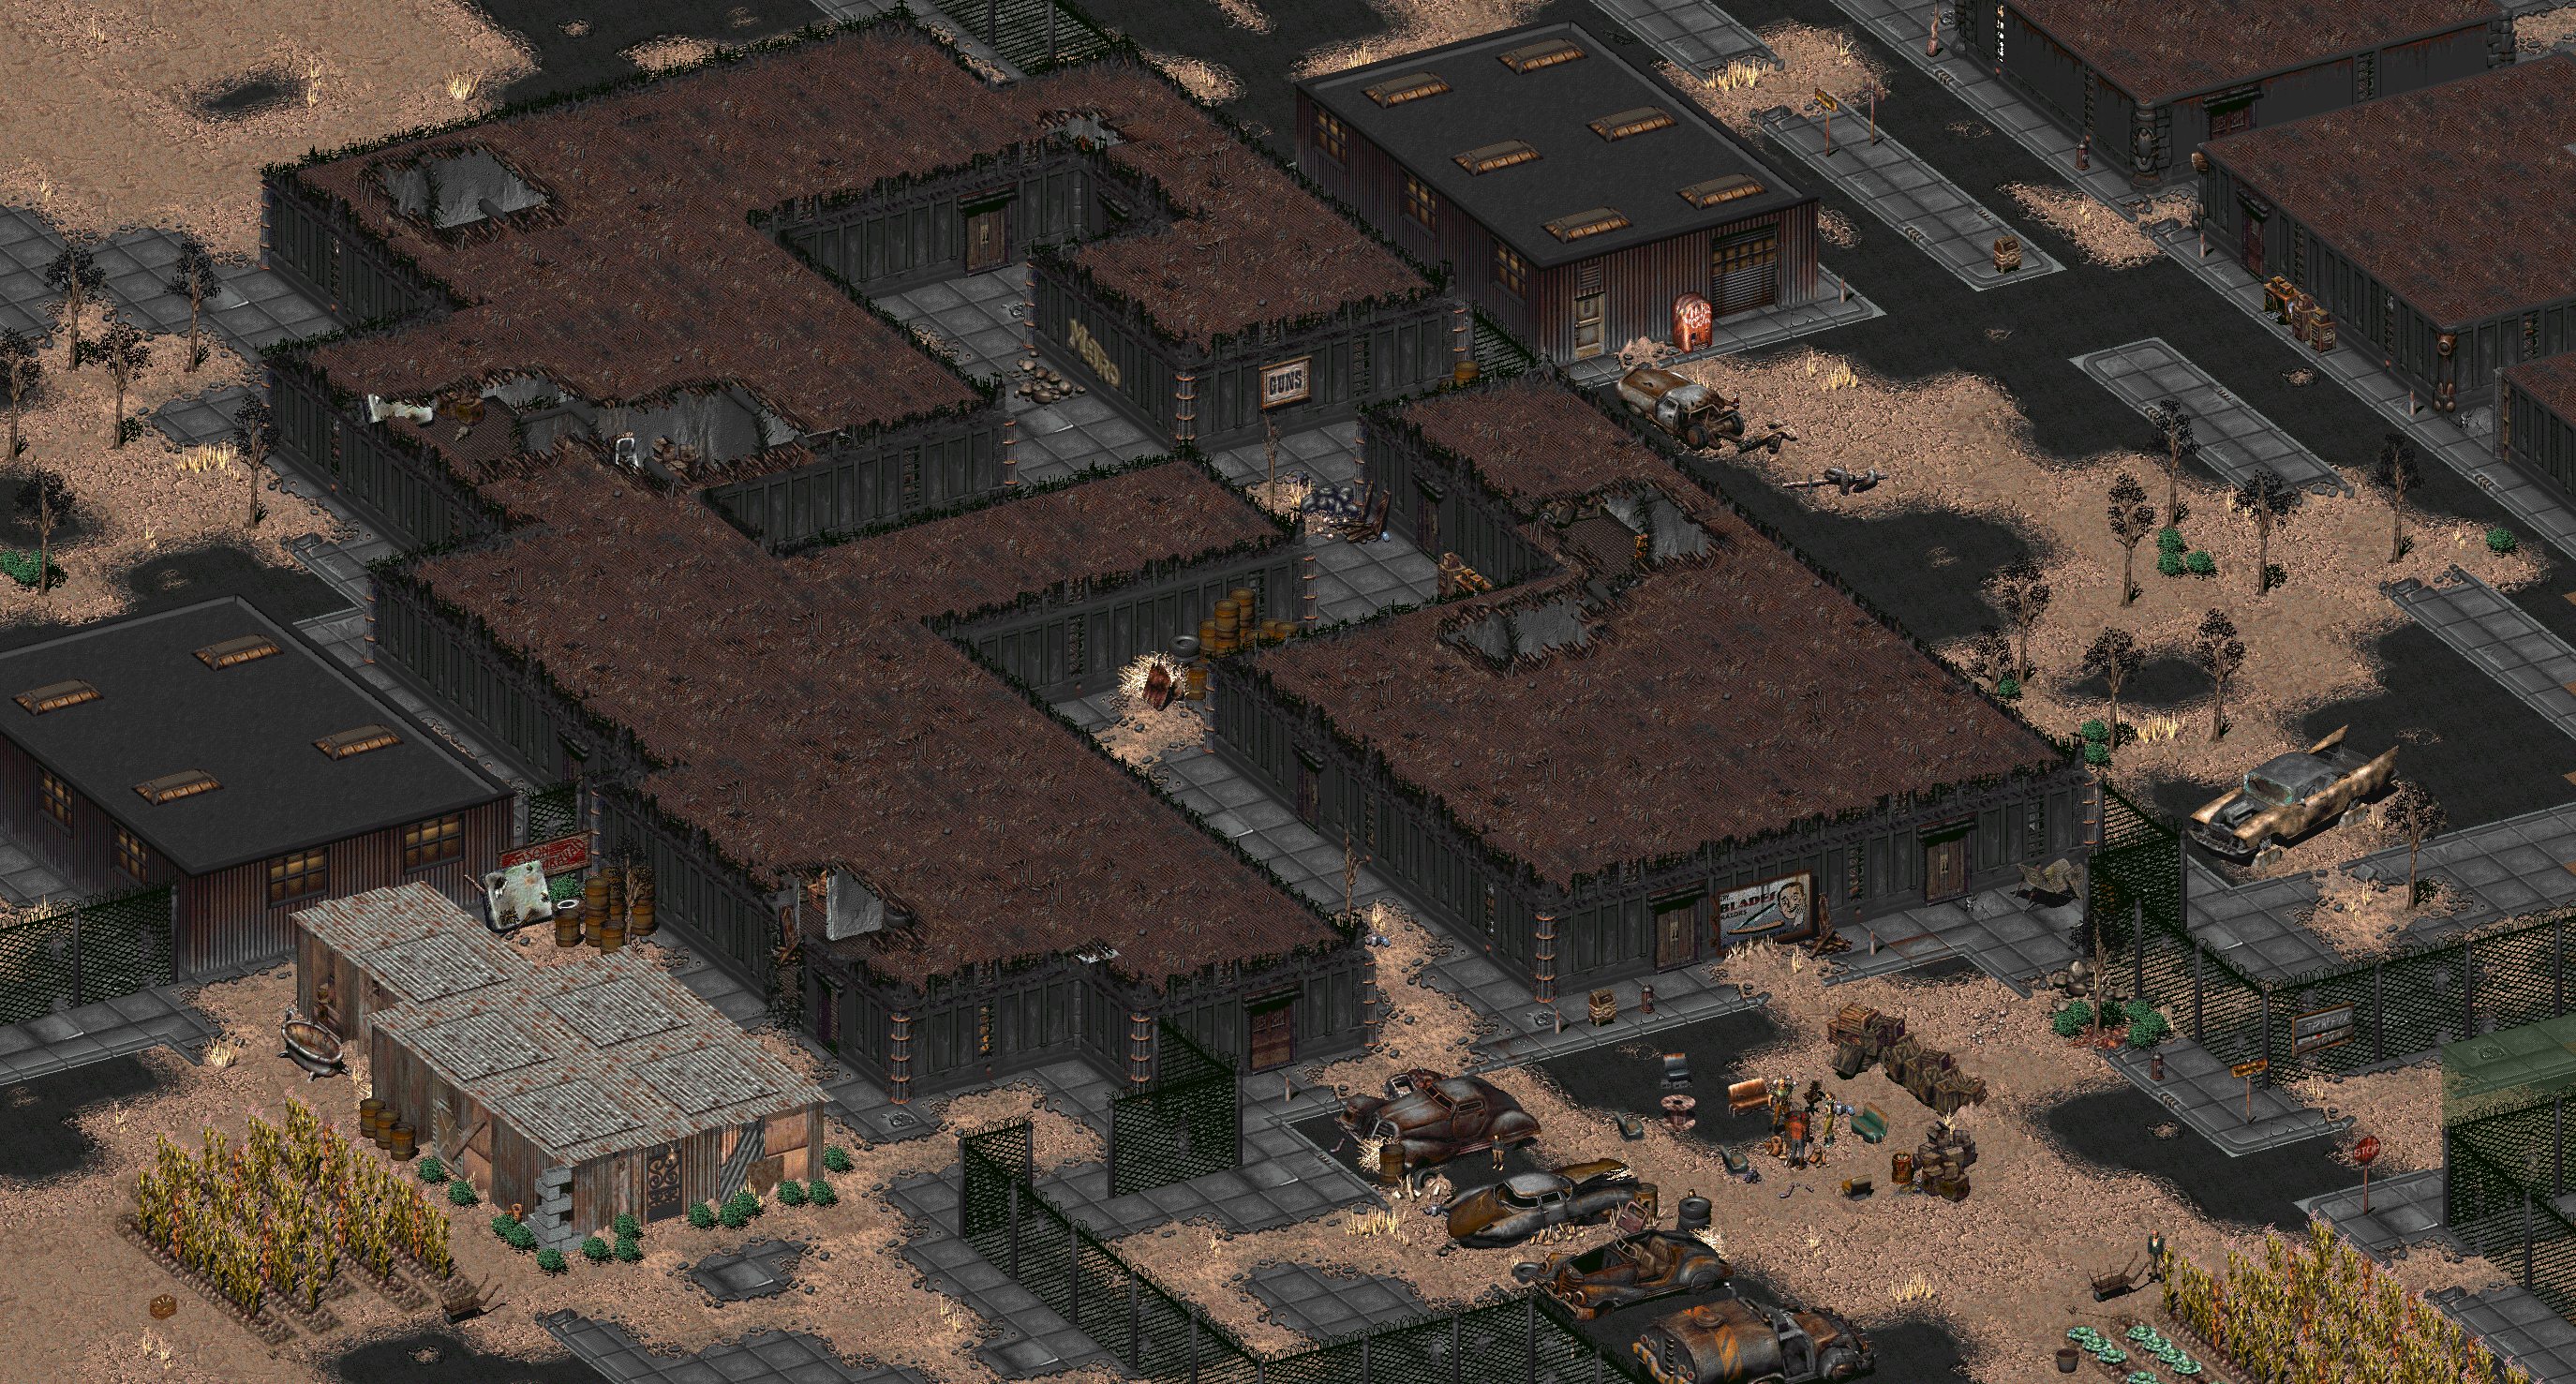
\includegraphics[width=1.0\textwidth]{fallout2}
        \end{minipage}
    \end{figure}
\end{frame}

\section{История развития}
\begin{frame}
    \frametitle{История развития}
    Вехи развития компьютерных игр:
    \begin{itemize}
        \item 1889 -- Фусадзиро Ямаути основал игровую компанию Marufuku по производству и 
            продаже игральных карт Ханафуда (ныне Nintendo).
        \item 1947 -- \emph{Ракетный симулятор} -- первое известное развлекательное средство, похожее на 
            компьютерную игру.
        \item 1948—1950 -- Алан Тьюринг и Дэйвид Чампернаун разработали алгоритм шахматной игры. 
        \item 1971 -- Биллом Питтсом создаётся первый аркадный автомат Galaxy Game на 
            базе PDP-11.
        \item 1975 -- Atari выходит на рынок игровых приставок с моделью Pong.
        \item 1978 -- Taito выпускает новый аркадный автомат Space Invaders.
    \end{itemize}
\end{frame}

\section{Классификация компьютерных игр}
\begin{frame}
    \frametitle{Классификация компьютерных игр}
    Классификация компьютерный игр по жанрам:
    \begin{itemize}
        \item Action (\emph{Space Invaders, Doom})\\
            \tiny Действие таких игр развивается очень динамично и требует напряжения внимания и 
            быстрой реакции на происходящие в игре события.
        \item \normalsize Adventure (\emph{Deponia, Monkey Island})\\
            \tiny Игра-повествование, в которой управляемый игроком герой продвигается по сюжету 
            и взаимодействует с игровым миром посредством применения предметов, общения с другими 
            персонажами и решения логических задач.
        \item \normalsize Arcade (\emph{Battle City, Mega Man})\\
            \tiny Игра, в которой игроку приходится действовать быстро, полагаясь в первую очередь 
            на свои рефлексы и реакцию.
        \item \normalsize Fighting (\emph{Mortal Kombat, Street Fighter})\\
            \tiny Геймплей состоит исключительно из поединков двух и более противников с применением 
            рукопашного боя.
        \item \normalsize FPS и TPS (\emph{Max Payne, Tomb Raider})\\
            \tiny В шутерах от первого лица (FPS) игрок не видит персонажа со стороны -- он наблюдает 
            за происходящим от лица персонажа -- <<глазами персонажа>>, и наблюдаемая игроком картина 
            совпадает с тем, что <<видит>> персонаж. В шутерах от третьего лица (TPS) игрок видит 
            персонаж со стороны с фиксированной или произвольной точки зрения.
    \end{itemize}
\end{frame}

\begin{frame}
    \frametitle{Классификация компьютерных игр}
    \begin{itemize}
        \item Hack and Slash (\emph{Diablo, Devil May Cry}) \\
            \tiny Игры с видом от третьего лица, основной частью игрового процесса, в которых 
            являются фехтовальные поединки с применением холодного и другого оружия.
        \item \normalsize Puzzle (\emph{Sokoban, Portal}) \\
            \tiny Название жанра компьютерных игр, целью которых является решение логических задач, 
            требующих от игрока задействования логики, стратегии и интуиции или в иных случаях 
            некоторого наличия удачи.
        \item \normalsize Rhythm game (\emph{Guitar Hero, Rock Band}) \\
            \tiny В музыкальных играх геймплей строится на взаимодействие игрока с музыкой. 
            Жанр же может быть любой, от головоломок до ритм игр.
        \item \normalsize RPG (\emph{Fallout, TES}) \\
            \tiny Жанр компьютерных игр, основанный на элементах игрового процесса традиционных 
            настольных ролевых игр.
        \item \normalsize RTS и TBS (\emph{Civilization, C\&C}) \\
            \tiny Игры, требующие планирования и выработки определенной стратегии для достижения 
            некоей конкретной цели, например, победы в военной операции.
        \item \normalsize Simulator (\emph{NFS, FIFA}) \\
            \tiny Игры, предоставляющие возможность симуляции и управления тем или иным процессом 
            из реальной жизни.
        \item \normalsize Traditional (\emph{карты, шашки}) \\
            \tiny Компьютерная реализация настольных игр.
    \end{itemize}
\end{frame}

\begin{frame}
    \frametitle{Классификация компьютерных игр}
    Так же существуют другие виды классификаций компьютерных игр:
    \begin{itemize}
        \item По платформе\\
            \tiny ПК, консоль, мобильное устройство, игровой автомат
        \item \normalsize По графическому изображению игры\\
            \tiny По расположению игровой камеры, по технологии графического изображения
        \item \normalsize По содержанию\\
            \tiny Жанр, сеттинг
        \item \normalsize По цели\\
            \tiny На прохождение, обучающая, казуальная, песочница, соревнование, хардкор
        \item \normalsize По издательским критериям\\
            \tiny <<ААА>>-класс, средний бюджет, Инди, любительская
        \item \normalsize По издательскому формату\\
            \tiny Оригинальная, игровая серия, дополнение, DLC
        \item \normalsize По типа распространения\\
            \tiny Физический, цифровой, shareware, free2play, бесплатная 
        \item \normalsize По количеству игроков\\
            \tiny Одиночная, совместная, многопользовательская, массовая
    \end{itemize}
\end{frame}

\section{Специализации разработчиков}
\begin{frame}
    \frametitle{Специализации разработчиков}
    В состав типичной современной команды разработчиков обычно входят представители разных 
    специализаций представленных ниже:
    \begin{figure}
        \begin{minipage}{0.55\textwidth}
            \begin{itemize}
                \item Графика\\
                    \tiny Арт-директор, 2D-художник, концепт-художник...
                \item \normalsize Дизайн\\
                    \tiny Ведущий дизайнер, дизайнер UI, сценарист...
                \item \normalsize Звук\\
                    \tiny Инженер по звуковым эффектам, композитор...
                \item \normalsize Контроль качества\\
                    \tiny QA локализации, бета-тест...
                \item \normalsize Программирование\\
                    \tiny Ведущий программист, программист AI...
                \item \normalsize Управление\\
                    \tiny Исполнительный продюсер, линейный продюсер.
            \end{itemize}
        \end{minipage}
        \begin{minipage}{0.40\textwidth}
            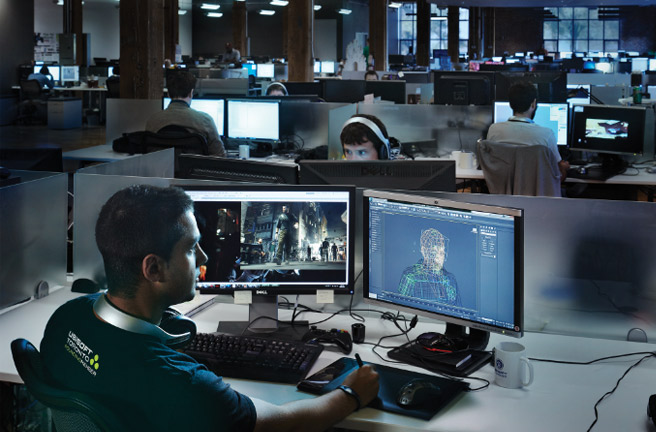
\includegraphics[width=1.0\textwidth]{ubisoft}\\
            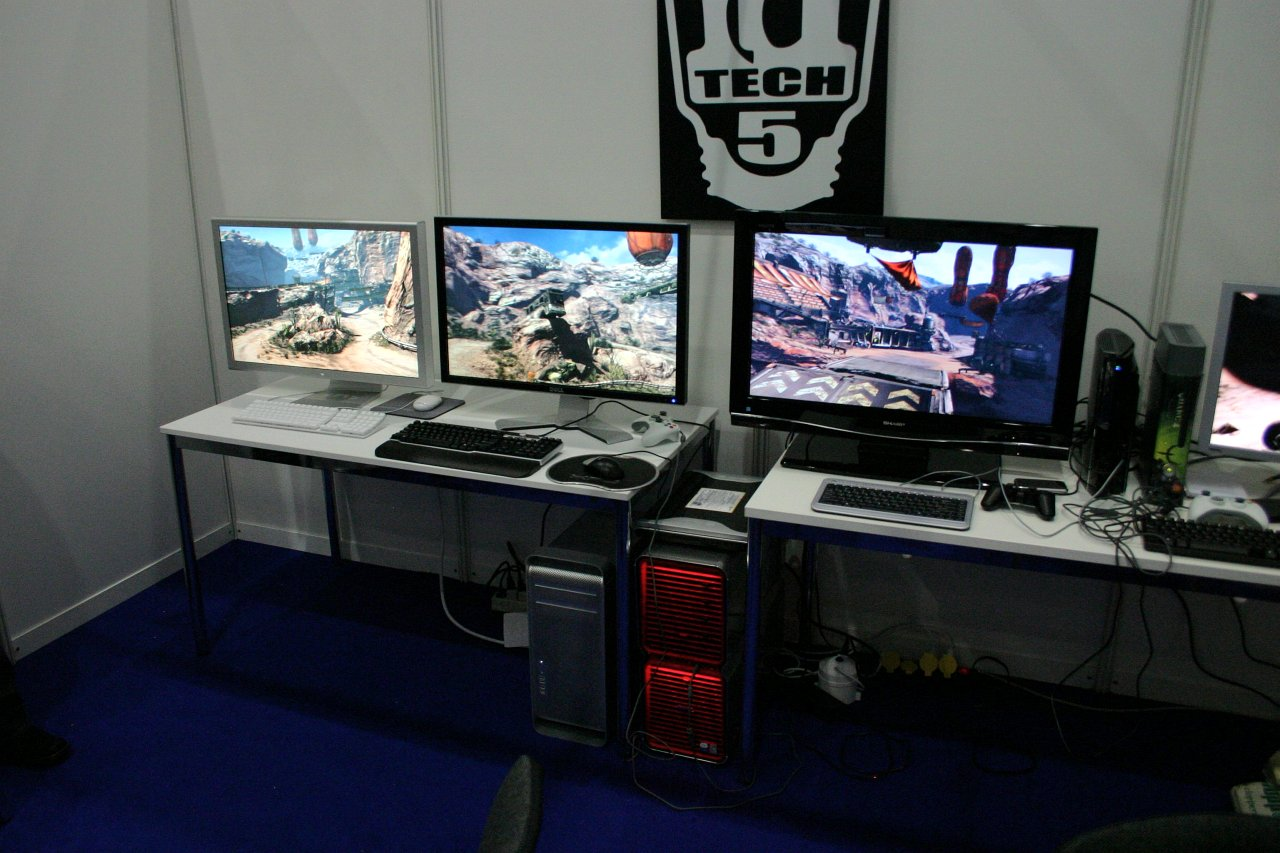
\includegraphics[width=1.0\textwidth]{id}
        \end{minipage}
    \end{figure}
\end{frame}

\section{Процесс разработки}
\begin{frame}
    \frametitle{Процесс разработки}
    Процесс разработки игры меняется в зависимости от компании и проекта. Однако разработка 
    коммерческой игры обычно включает следующие стадии:
    \begin{figure}
        \begin{minipage}{0.47\textwidth}
            \begin{itemize}
                \item Предпроизводственный процесс
                \item Производство
                \item Поддержка
            \end{itemize}
        \end{minipage}
        \begin{minipage}{0.5\textwidth}
            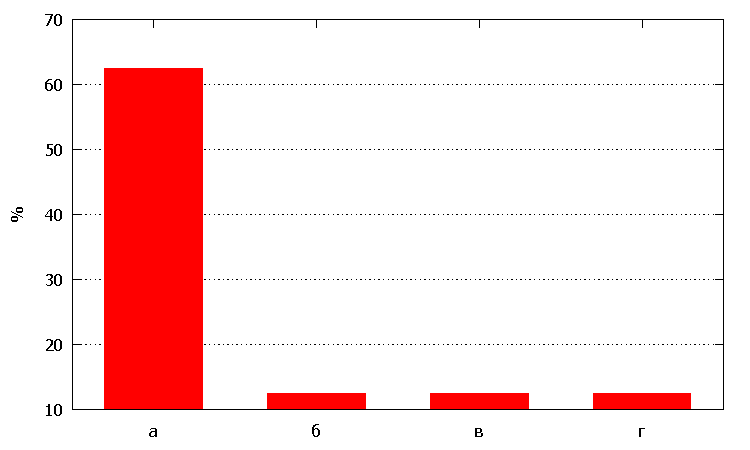
\includegraphics[width=1.0\textwidth]{work}
        \end{minipage}
    \end{figure}
\end{frame}

\begin{frame}
    \frametitle{Процесс разработки}
    \framesubtitle{Предпроизводственный процесс}
    Предпроизводственный процесс включает в себя следующие пункты:
    \begin{figure}
        \begin{minipage}{0.47\textwidth}
            \begin{itemize}
                \item Формирование идеи
                \item Определение жанра
                \item Создание геймплея
                \item Эскизный проект
                \item Документация проектировщика
            \end{itemize}
        \end{minipage}
        \begin{minipage}{0.5\textwidth}
            
\includegraphics[width=1.0\textwidth]{idea}
        \end{minipage}
    \end{figure}
\end{frame}

\begin{frame}
    \frametitle{Процесс разработки}
    \framesubtitle{Производственный процесс}
    Производственный процесс состоит из работы над:
    \begin{figure}
        \begin{minipage}{0.47\textwidth}
            \begin{itemize}
                \item Процесс разработки
                \begin{itemize}
                    \item Программирование
                    \item Графика
                    \item Дизайн
                    \item Эффекты
                    \item Звук
                \end{itemize}
                \item Контроль качества
                \item Управление разработкой
            \end{itemize}
        \end{minipage}
        \begin{minipage}{0.5\textwidth}
            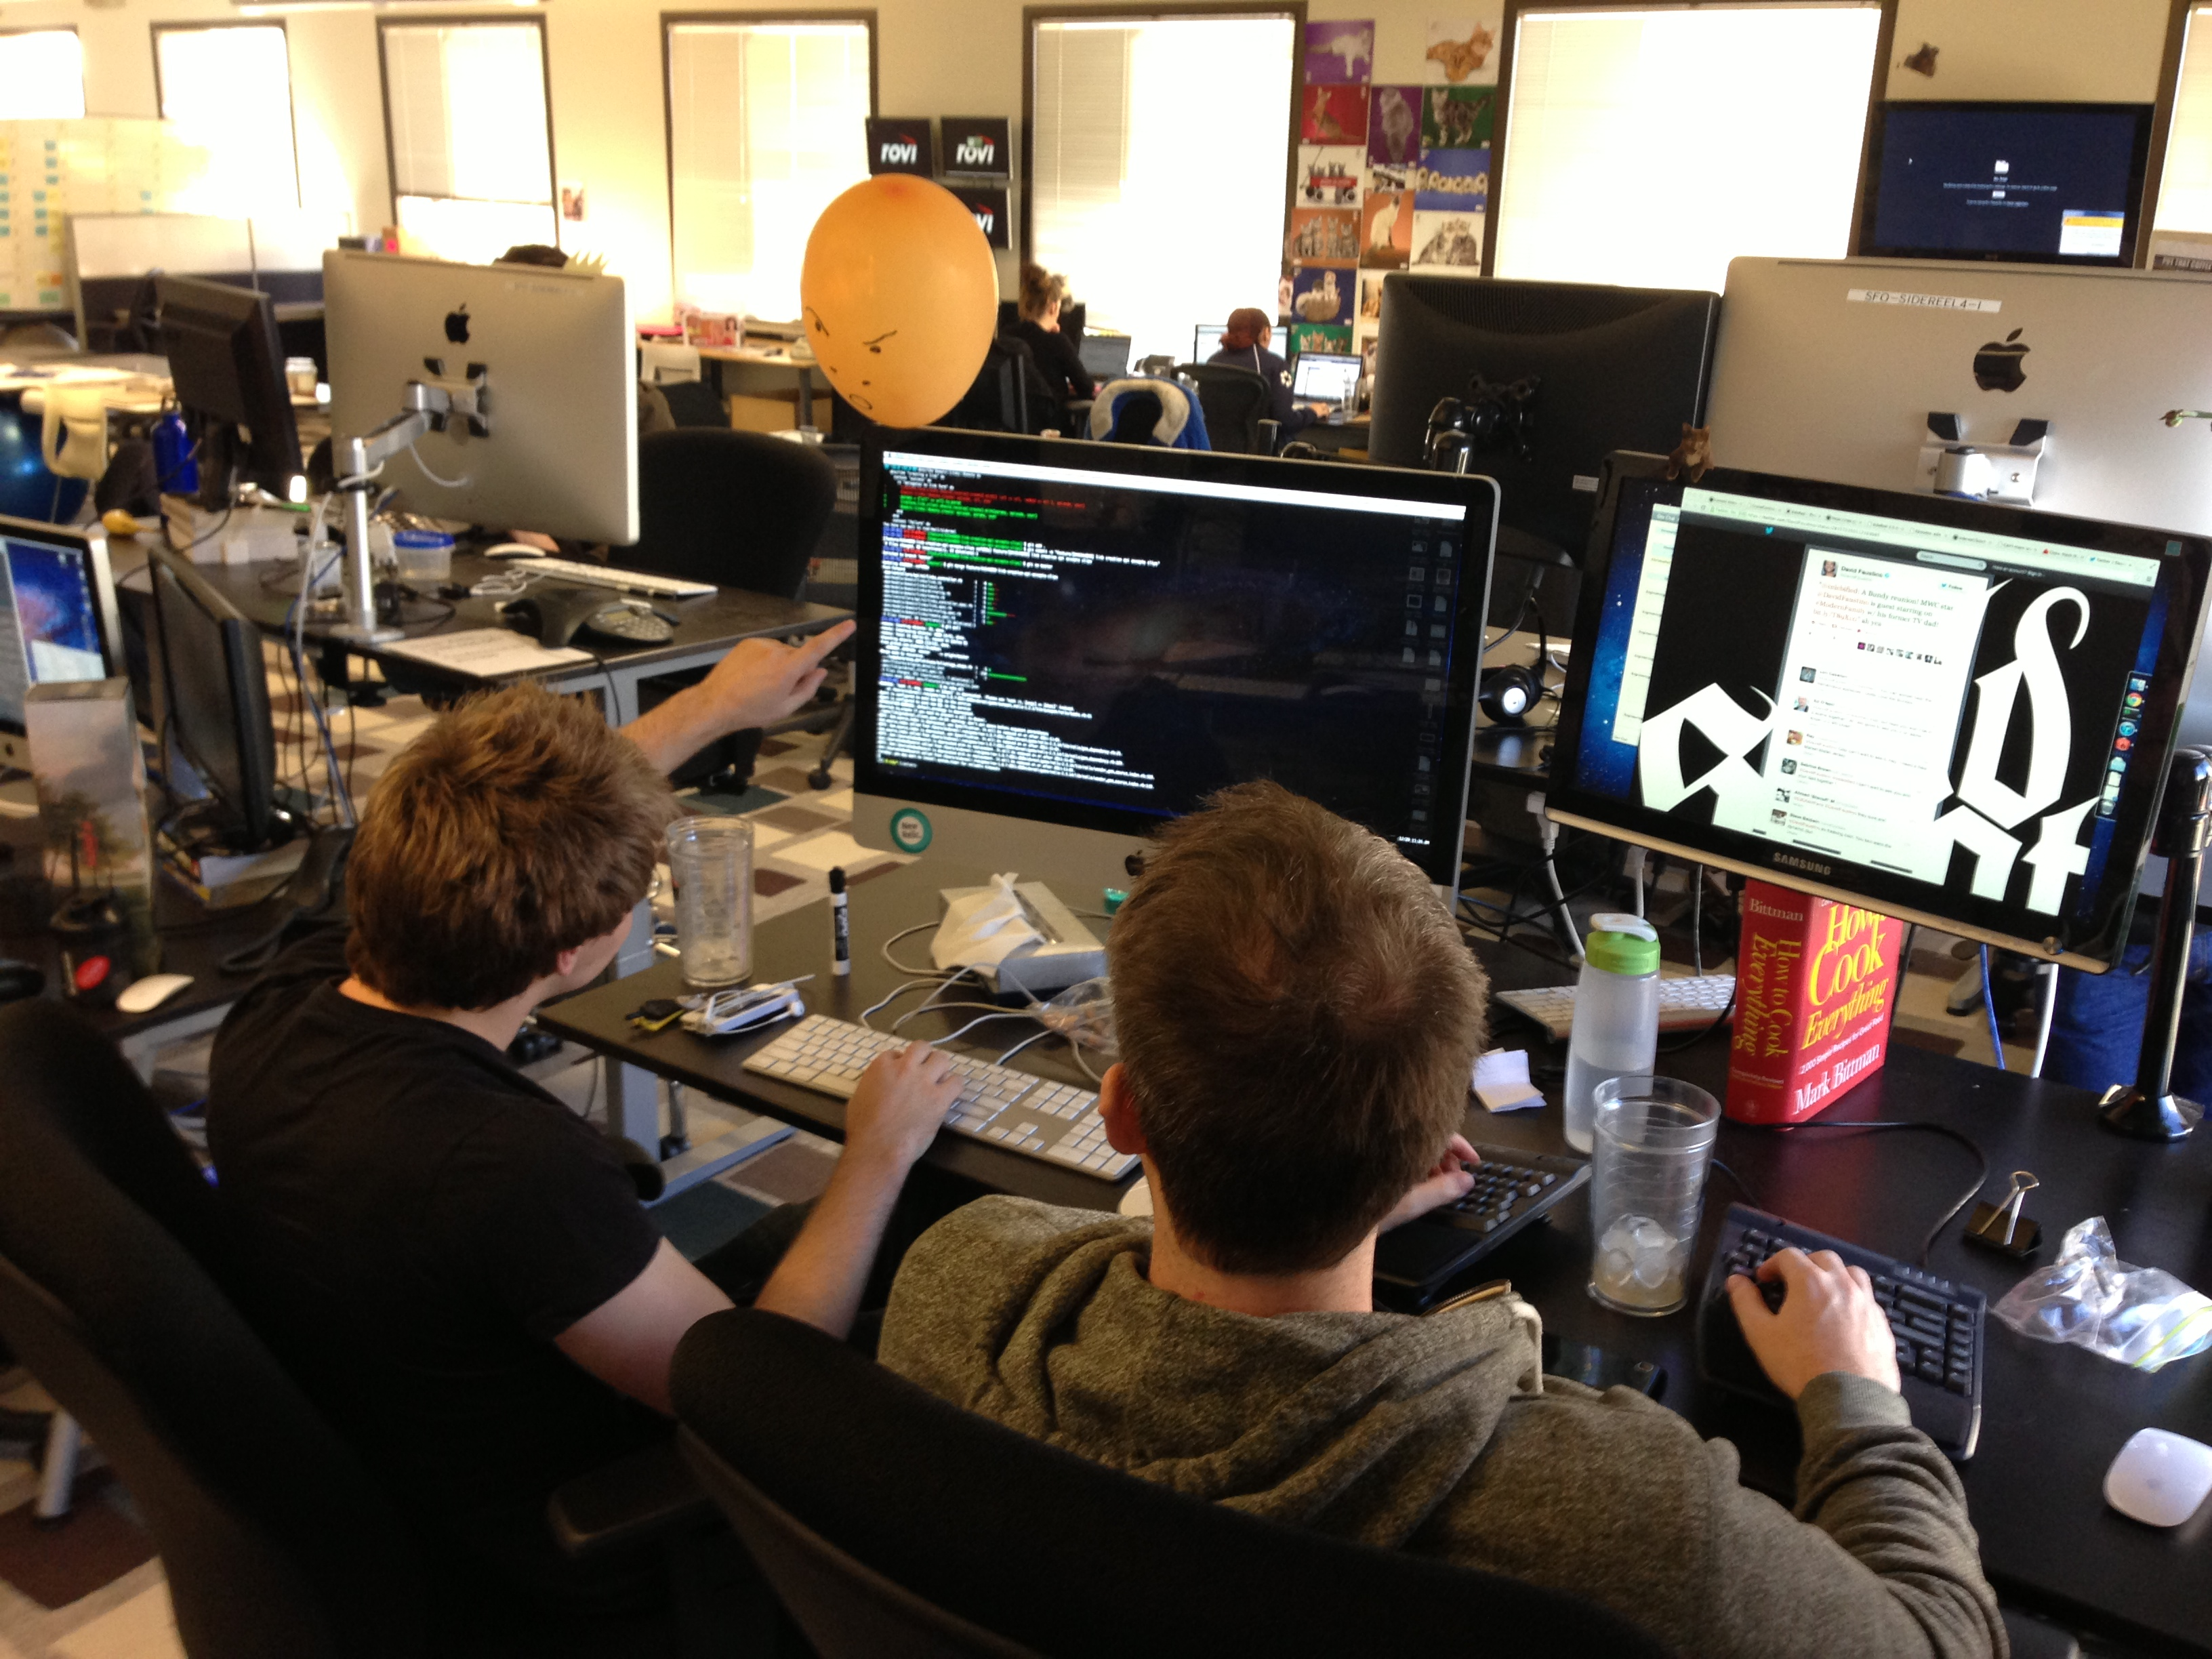
\includegraphics[width=1.0\textwidth]{programming}
        \end{minipage}
    \end{figure}
\end{frame}

\begin{frame}
    \frametitle{Процесс разработки}
    \framesubtitle{Процесс поддержки}
    Поддержка готового продукта состоит из:
    \begin{figure}
        \begin{minipage}{0.47\textwidth}
            \begin{itemize}
                \item Исправление ошибок и выпуск патчей
                \item Расширение игровой функциональности
                \item Выпуск дополнений
                \item Выпуск DLC
            \end{itemize}
        \end{minipage}
        \begin{minipage}{0.5\textwidth}
            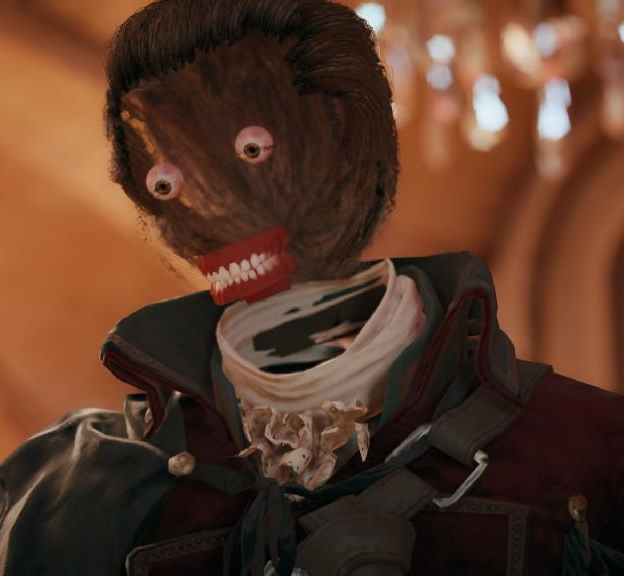
\includegraphics[width=1.0\textwidth]{bugs}
        \end{minipage}
    \end{figure}
\end{frame}

\section{Аутсорсинг}
\begin{frame}
    \frametitle{Аутсорсинг}
    Планы касательно аутсорсинга рассматривают на этапе подготовки производства; именно тогда 
    рассчитывают необходимые временные и финансовые затраты на работу, которая будет произведена вне 
    компании-разработчика.
    \begin{figure}
        \begin{minipage}{0.47\textwidth}
            \begin{itemize}
                \item Модульные инструменты
                \item Музыкальные треки
                \item Актёрская озвучка
                \item Захват движений
            \end{itemize}
        \end{minipage}
        \begin{minipage}{0.5\textwidth}
            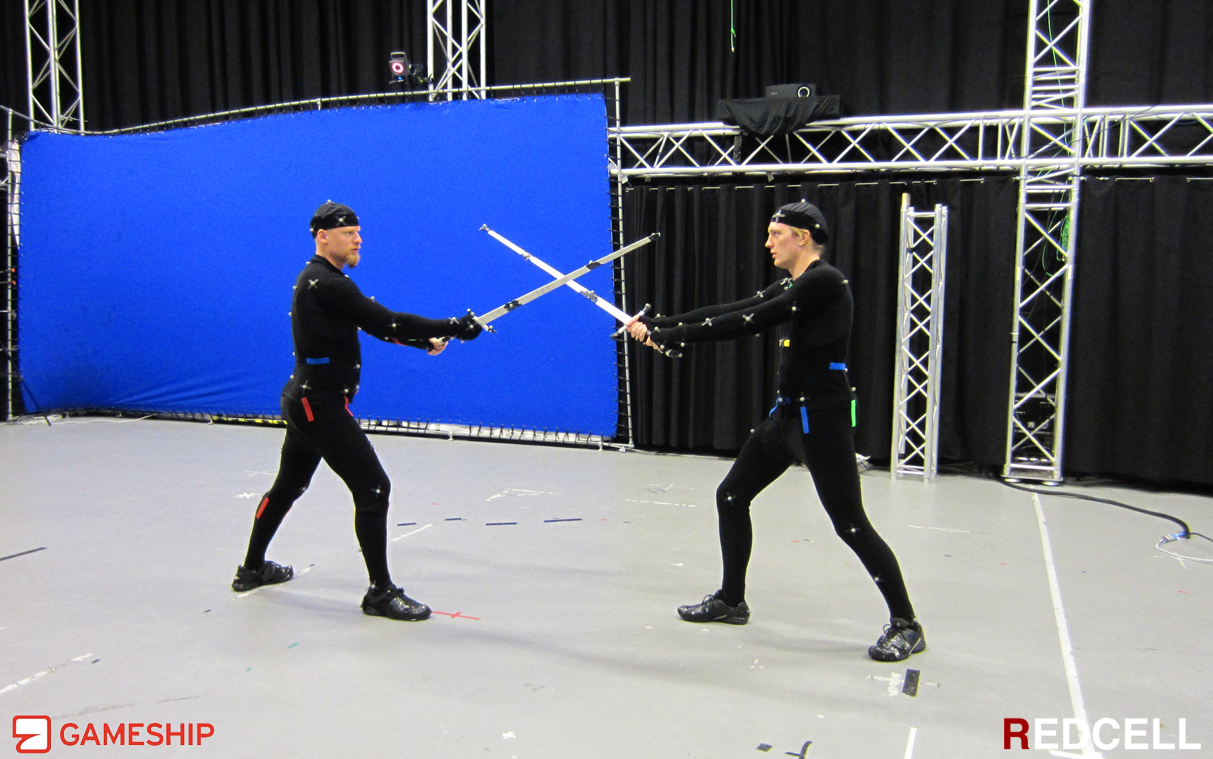
\includegraphics[width=1.0\textwidth]{mocap}
        \end{minipage}
    \end{figure}
\end{frame}

\section{Перспективность}
\begin{frame}
    \frametitle{Перспективность}
    \begin{itemize}
        \item Пример удачных инди проектов
        \begin{itemize}
            \item \emph{FEZ} (\url{http://fezgame.com/})
            \item \emph{Minecraft} (\url{https://minecraft.net/})
            \item \emph{Super Meat Boy} (\url{http://})
            \item \emph{World of Goo} (\url{http://worldofgoo.com/})
        \end{itemize}
        \item Использования цифровой дистрибуции
        \begin{itemize}
            \item Steam
            \item GOG
            \item Origin
            \item UPlay
        \end{itemize}
        \item Доступность информации и инструментов
        \item Соревновая по разработке
        \item Большой выбор платформ
    \end{itemize}
\end{frame}

\section{Список источников}
\begin{frame}
    \frametitle{Список источников}
    Где почитать по теме:
    \begin{itemize}
        \item \url{http://www.dtf.ru/}
        \item \url{http://www.gamedev.net/}
        \item \url{http://www.gamedev.ru/}
        \item \url{http://www.habrahabr.ru/}
        \item \url{http://www.kotaku.com/}
        \item \url{http://www.gamasutra.com/}
        \item \url{http://www.gamedaily.com/}
        \item \url{http://www.ign.com/}
    \end{itemize}
\end{frame}

\begin{frame}
    \Huge\centeringСпасибо за внимание!
\end{frame}